\documentclass[a4paper,11pt]{article}

%%%%%%%%%%%%%%%%%%%%%%%%%%%%%%%%%
%    PACKAGES AND DEFINITIONS   %
%%%%%%%%%%%%%%%%%%%%%%%%%%%%%%%%%
\usepackage{amssymb}
\usepackage{amsmath}
\usepackage{epsfig}
\usepackage{booktabs}
\usepackage{subfig}

\usepackage{fancyhdr}
\usepackage{lastpage}
\usepackage{verbatim}
\usepackage[usenames,dvipsnames]{color}
\usepackage[hyperindex, linktocpage]{hyperref}
\usepackage[english]{babel}
\usepackage{fullpage}
\usepackage{graphicx}

\usepackage[final]{listings}
\usepackage{color}

\lstloadlanguages{[GNU]C++}
\lstset{
    frameround=fttt,
    language=[GNU]C++,
    numbers=left,
    breaklines=true,
    keywordstyle=\color{blue}\bfseries, 
    basicstyle=\ttfamily\color{black},
    numberstyle=\color{black}
}

\usepackage{indentfirst}

\newcommand{\class}{Computer Vision}
\newcommand{\expT}{Object recognition and tracking}
\newcommand{\cand}{Giovanni Fregonese ID 1232107; email: giovanni.fregonese@studenti.unipd.it \\
                   Emilio Olivastri ID ; email: emilio.olivastri@studenti.unipd.it}
\newcommand{\dateD}{June 4th 2020}


\begin{document}

\begin{center}
	\Large
	\begin{center}
		\textsl{Laboratory 6: \expT}\\
		\large
		\hfill\break
		\textsl{\cand}\\
		\dateD
	\end{center}
\end{center}

\subsection*{Activity Goal}



\subsection*{Lesson Learned}



\subsection*{Personal Considerations}


\begin{figure}[h]
    \centering
    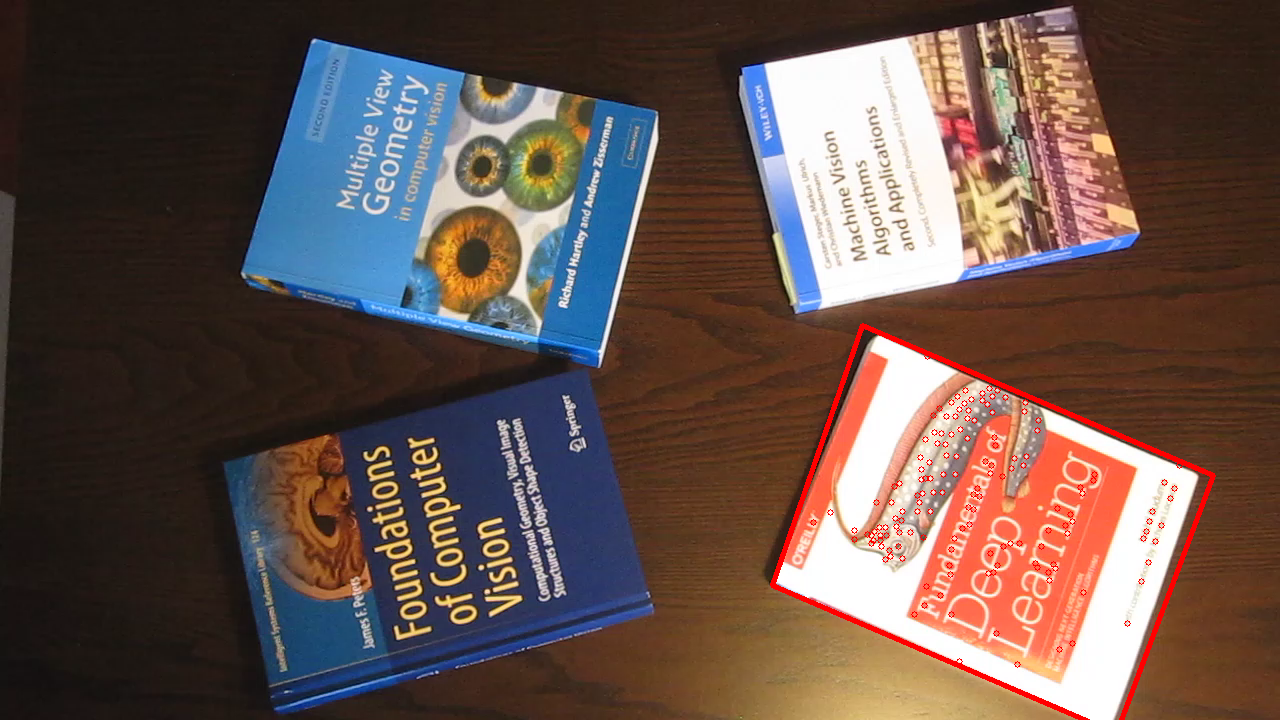
\includegraphics[width=\textwidth]{imgs/TrackedFeatures0.png}
    \caption{Tracked book 1}
    \label{fig:book1}
\end{figure}

\begin{figure}[h]
    \centering
    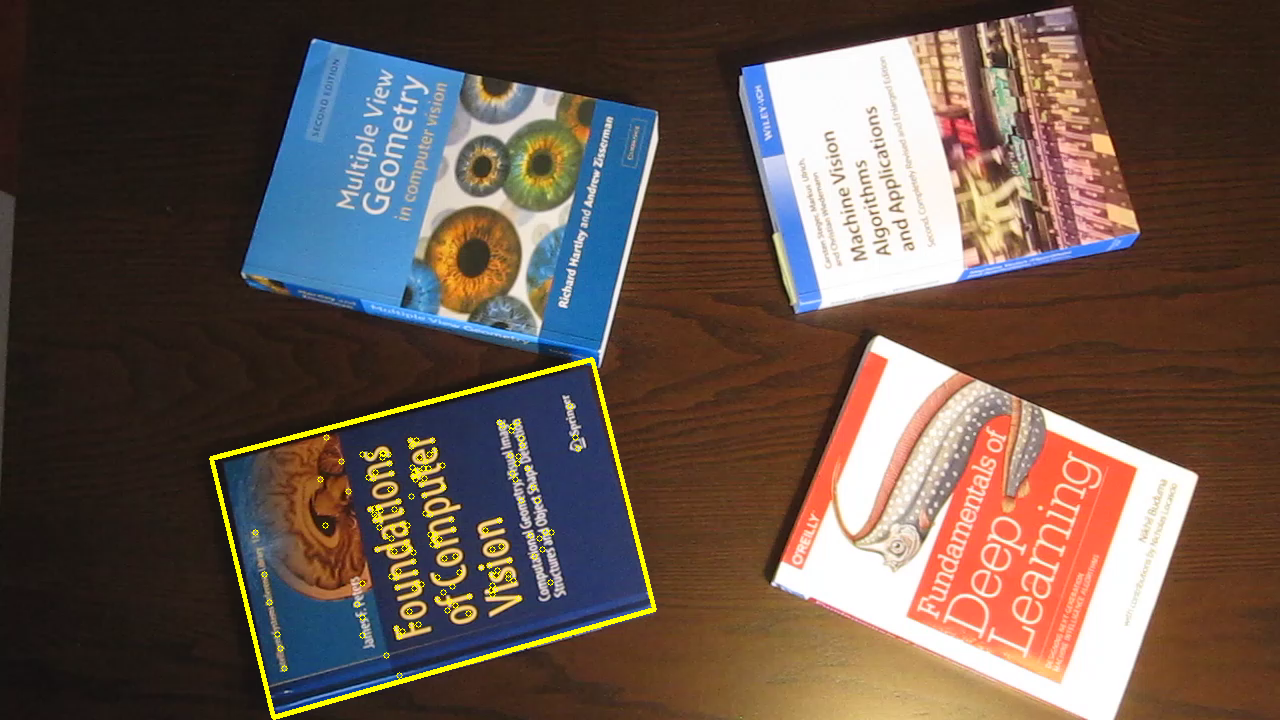
\includegraphics[width=\textwidth]{imgs/TrackedFeatures1.png}
    \caption{Tracked book 2}
    \label{fig:book2}
\end{figure}

\begin{figure}[h]
    \centering
    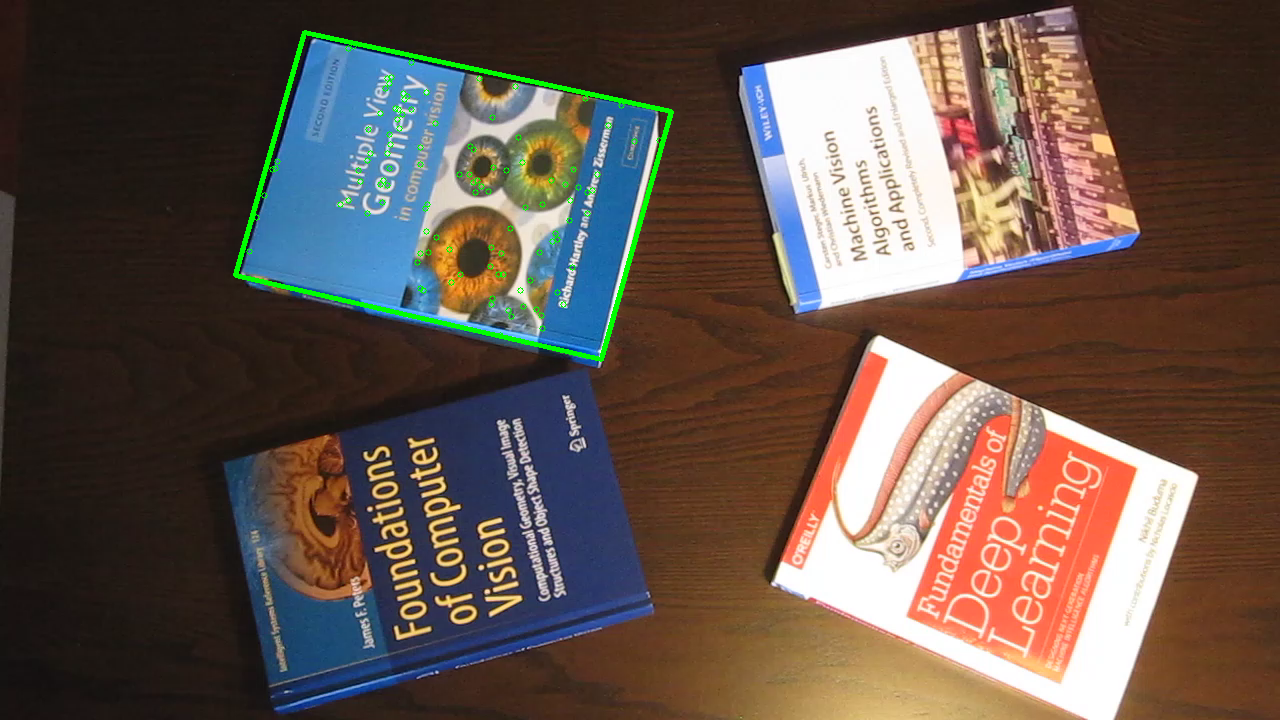
\includegraphics[width=\textwidth]{imgs/TrackedFeatures2.png}
    \caption{Tracked book 3}
    \label{fig:book3}
\end{figure}

\begin{figure}[h]
    \centering
    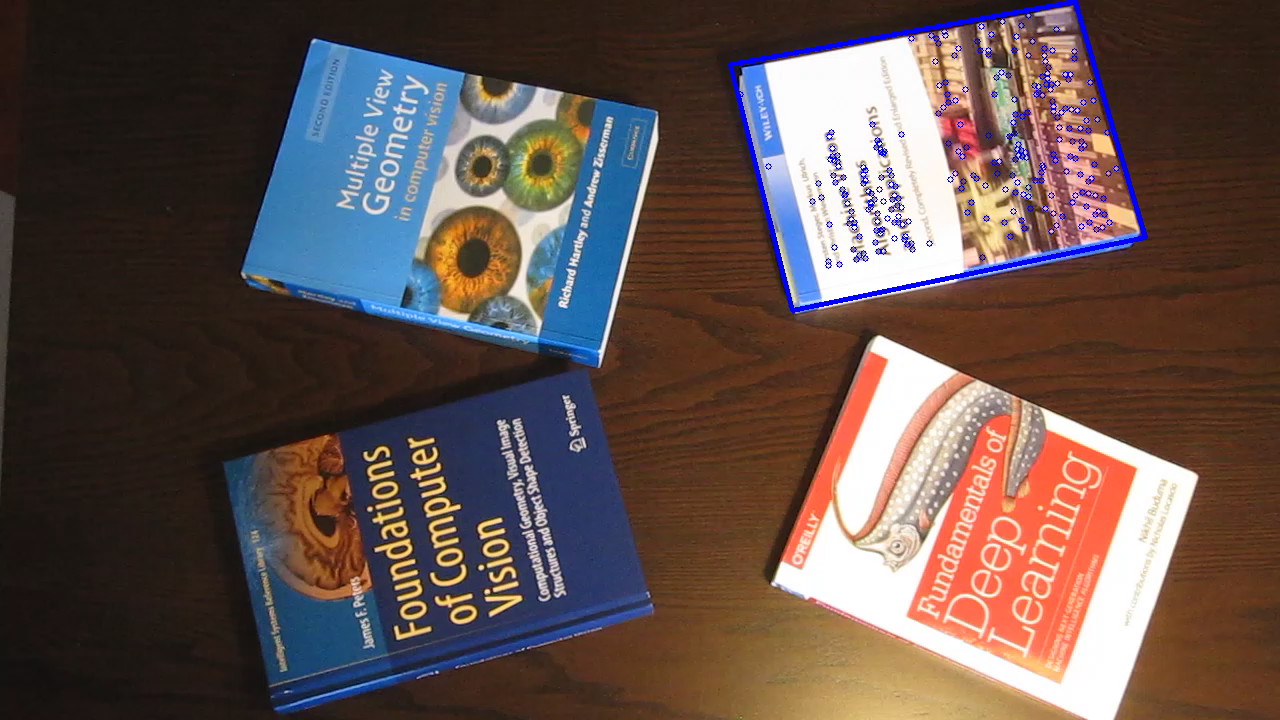
\includegraphics[width=\textwidth]{imgs/TrackedFeatures3.png}
    \caption{Tracked book 4}
    \label{fig:book4}
\end{figure}

\end{document}